\documentclass[12pt]{article}
\usepackage[margin = 1in]{geometry}
\usepackage{amsmath}
\usepackage{amssymb}
\usepackage{graphicx}
\usepackage{subfig}
\usepackage{cancel}

\begin{document}
	
	\begin{center}
		\textbf{Homework 2} \\
		\textbf{Numerical Matrix Analysis} \\
		\textbf{Math 543} \\
		\textbf{Stephen Giang} \\
	\end{center}

\noindent \textbf{Exercise 4.1: } Determine the SVD's of the following matrices. \\
$$
	a. \begin{bmatrix}
			3 & 0 \\
			0 & -2
		\end{bmatrix} \qquad
	b. \begin{bmatrix}
			2 & 0 \\
			0 & 3
		\end{bmatrix} \qquad
	c. \begin{bmatrix}
			0 & 2 \\
			0 & 0 \\
			0 & 0	
		\end{bmatrix} \qquad
	d. \begin{bmatrix}
			1 & 1 \\
			0 & 0 
		\end{bmatrix} \qquad
	e. \begin{bmatrix}
			1 & 1 \\
			1 & 1		
		\end{bmatrix}
$$
\textbf{Solution Exercise 4.1: } \\\\
$$
	a. \begin{bmatrix}
			3 & 0 \\
			0 & -2
		\end{bmatrix} =
		\begin{bmatrix}
			1 & 0 \\
			0 & 1 
		\end{bmatrix}
		\begin{bmatrix}
			3 & 0 \\
			0 & 2 
		\end{bmatrix}
		\begin{bmatrix}
			1 & 0 \\
			0 & -1 
		\end{bmatrix}^*		
$$ \\
$$
	b. \begin{bmatrix}
			2 & 0 \\
			0 & 3
		\end{bmatrix} =
		\begin{bmatrix}
			0 & 1 \\
			1 & 0 
		\end{bmatrix}
		\begin{bmatrix}
			3 & 0 \\
			0 & 2 
		\end{bmatrix}
		\begin{bmatrix}
			0 & 1 \\
			1 & 0 
		\end{bmatrix}^*		
$$ \\
$$
	c. \begin{bmatrix}
			0 & 2 \\
			0 & 0 \\
			0 & 0
		\end{bmatrix} =
		\begin{bmatrix}
			1 & 0 & 0 \\
			0 & 1 & 0 \\
			0 & 0 & 1
		\end{bmatrix}
		\begin{bmatrix}
			2 & 0 \\
			0 & 0 \\
			0 & 0
		\end{bmatrix}
		\begin{bmatrix}
			0 & -1 \\
			1 & 0 
		\end{bmatrix}^*			
$$ \\
$$
	d. \begin{bmatrix}
			1 & 1 \\
			0 & 0
		\end{bmatrix} =
		\begin{bmatrix}
			1 & 0 \\
			0 & 1 
		\end{bmatrix}
		\begin{bmatrix}
			1.4142 & 0 \\
			0 & 0 
		\end{bmatrix}
		\begin{bmatrix}
			.7071 & -.7071 \\
			.7071 & .7071 
		\end{bmatrix}^*		
$$ \\
$$
	e. \begin{bmatrix}
			1 & 1 \\
			1 & 1
		\end{bmatrix} =
		\begin{bmatrix}
			-.7071 & -.7071 \\
			-.7071 & .7071 
		\end{bmatrix}
		\begin{bmatrix}
			2 & 0 \\
			0 & 0 
		\end{bmatrix}
		\begin{bmatrix}
			-.7071 & .7071 \\
			-.7071 & -.7071 
		\end{bmatrix}^*			
$$ \\
\newpage
\noindent \textbf{Exercise 4.3: } Write a MATLAB program (see Lecture 9) which, given a real 2 x 2
matrix $\mathbb{A}$, plots the right singular vectors $v_1$ and $v_2$ in the unit circle and also
the left singular vectors $u_1$ and $u_2$ in the appropriate ellipse, as in Figure 4.1.
Apply your program to the matrix (3.7) and also to the 2 x 2 matrices of Exercise 4.1. ||
$\text{Matrix 3.7: }
	\begin{bmatrix}
		1 & 2 \\
		0 & 2
	\end{bmatrix}
$ \\
	\begin{figure}[h!]
		\centering
		\subfloat[Matrix 3.7]{{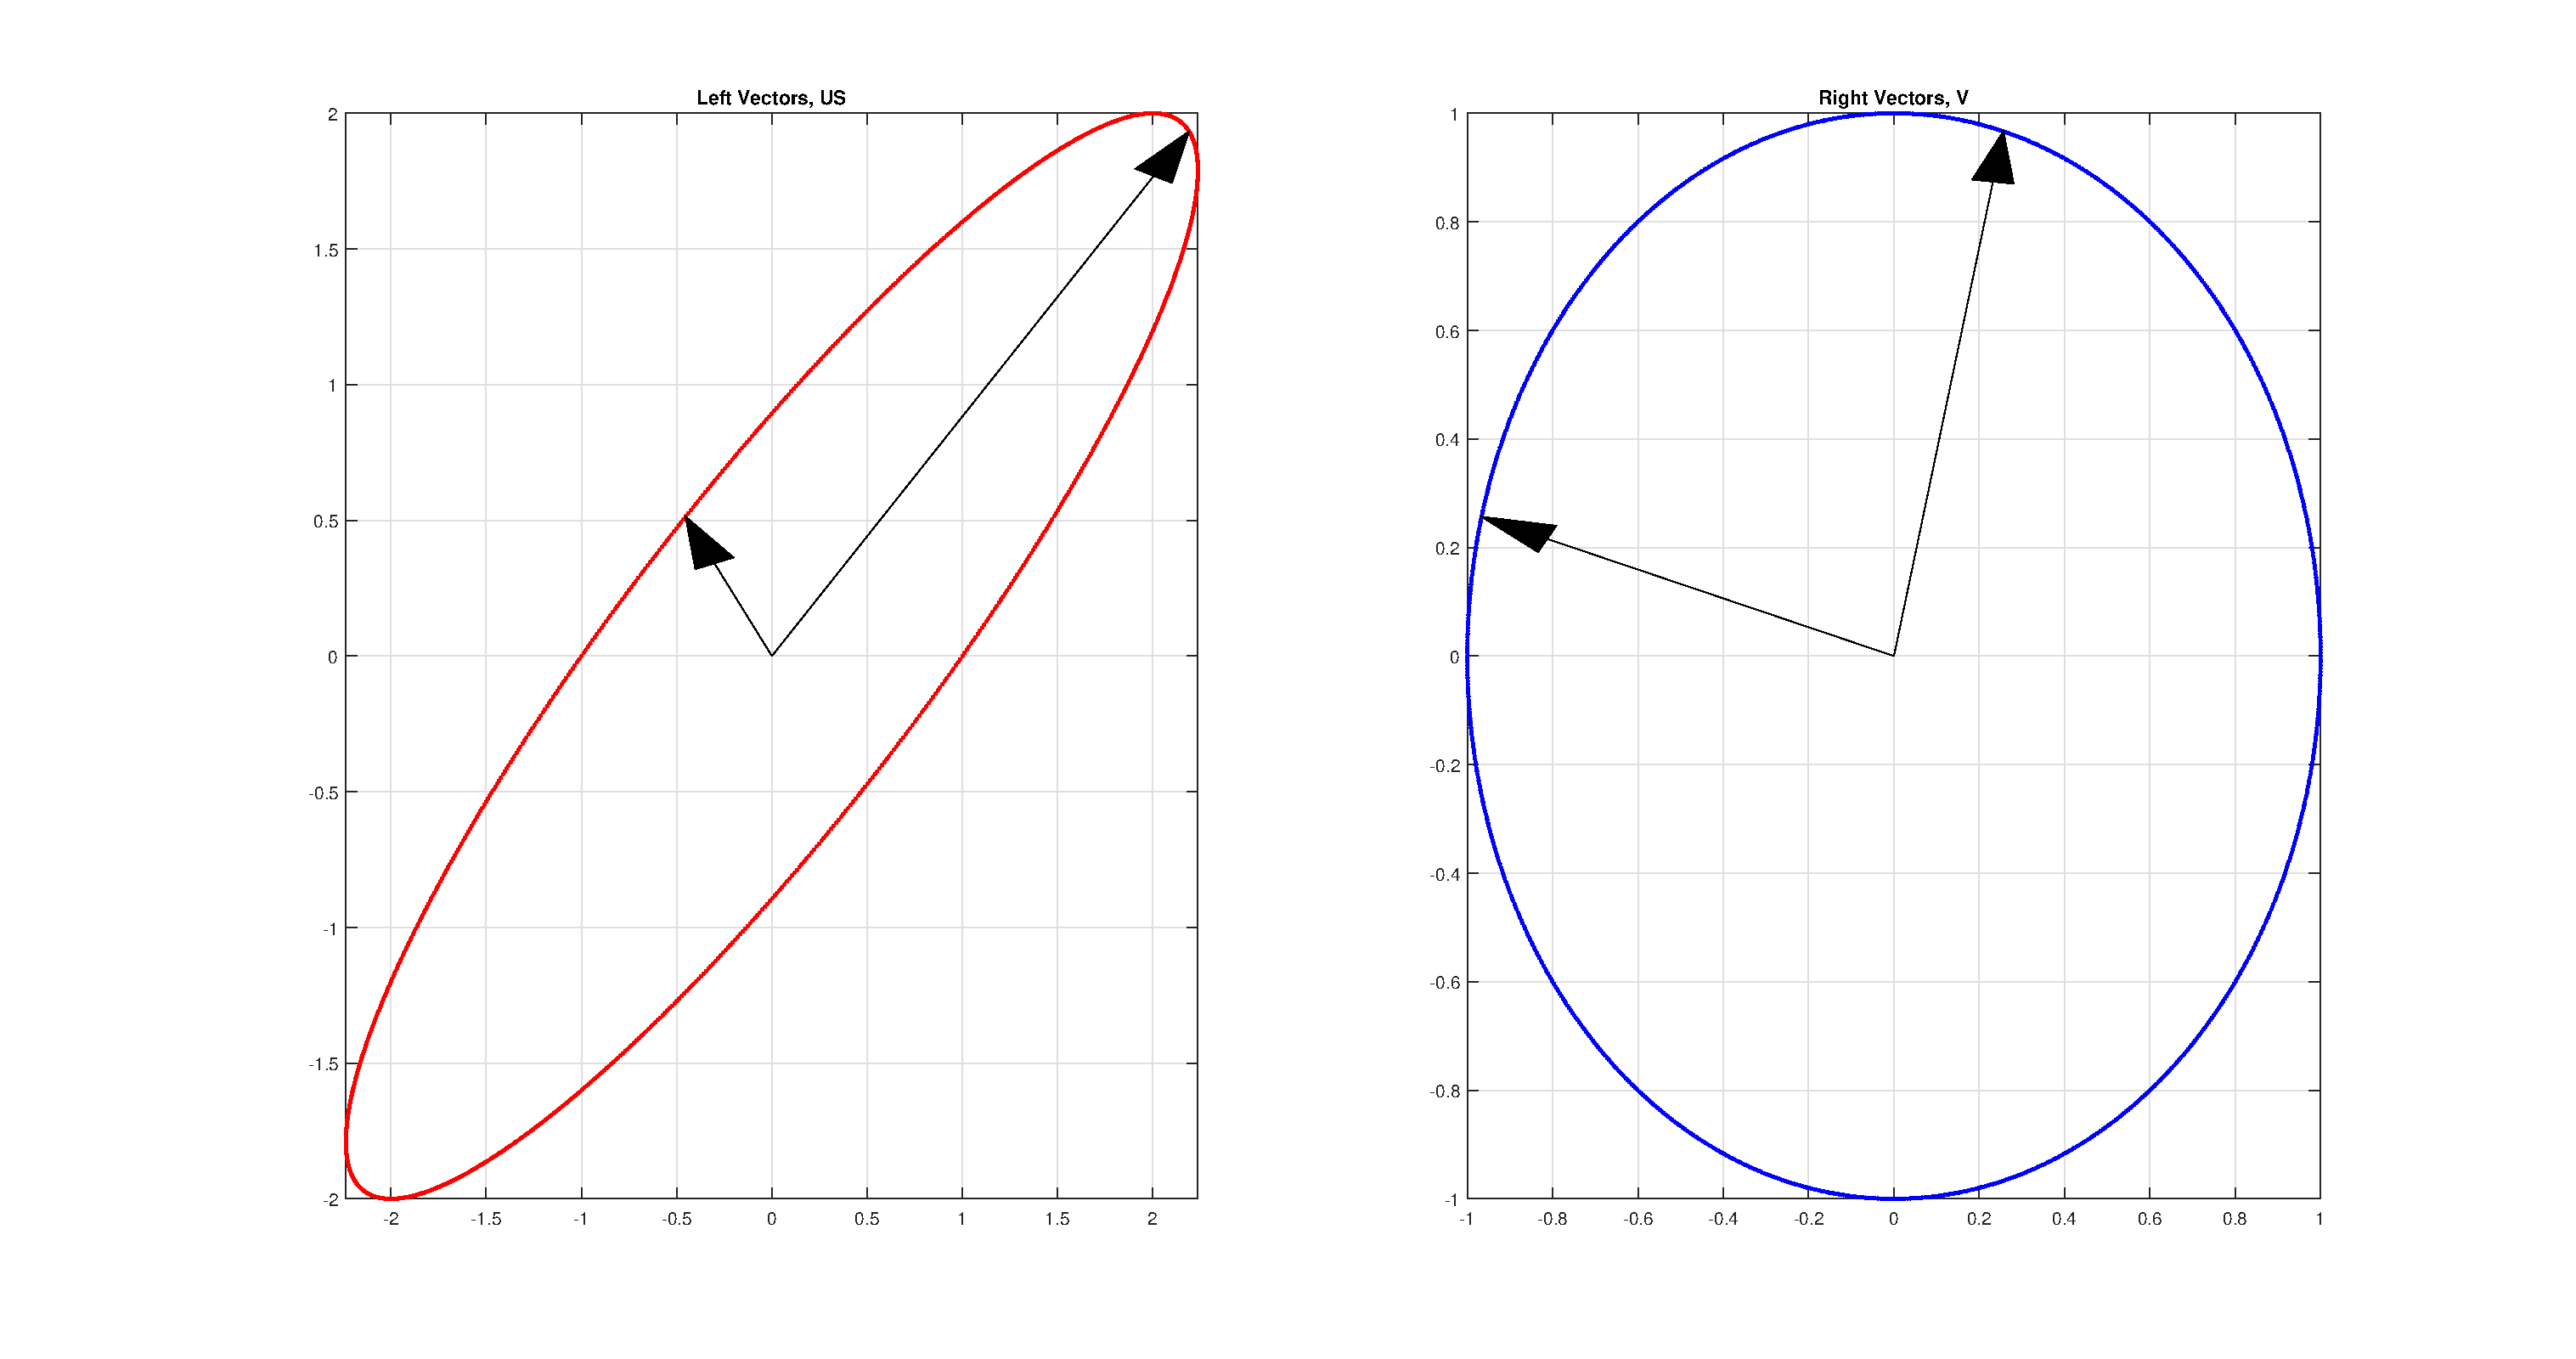
\includegraphics[width=9cm] {Matrix37} }}
		\subfloat[Matrix (a)]{{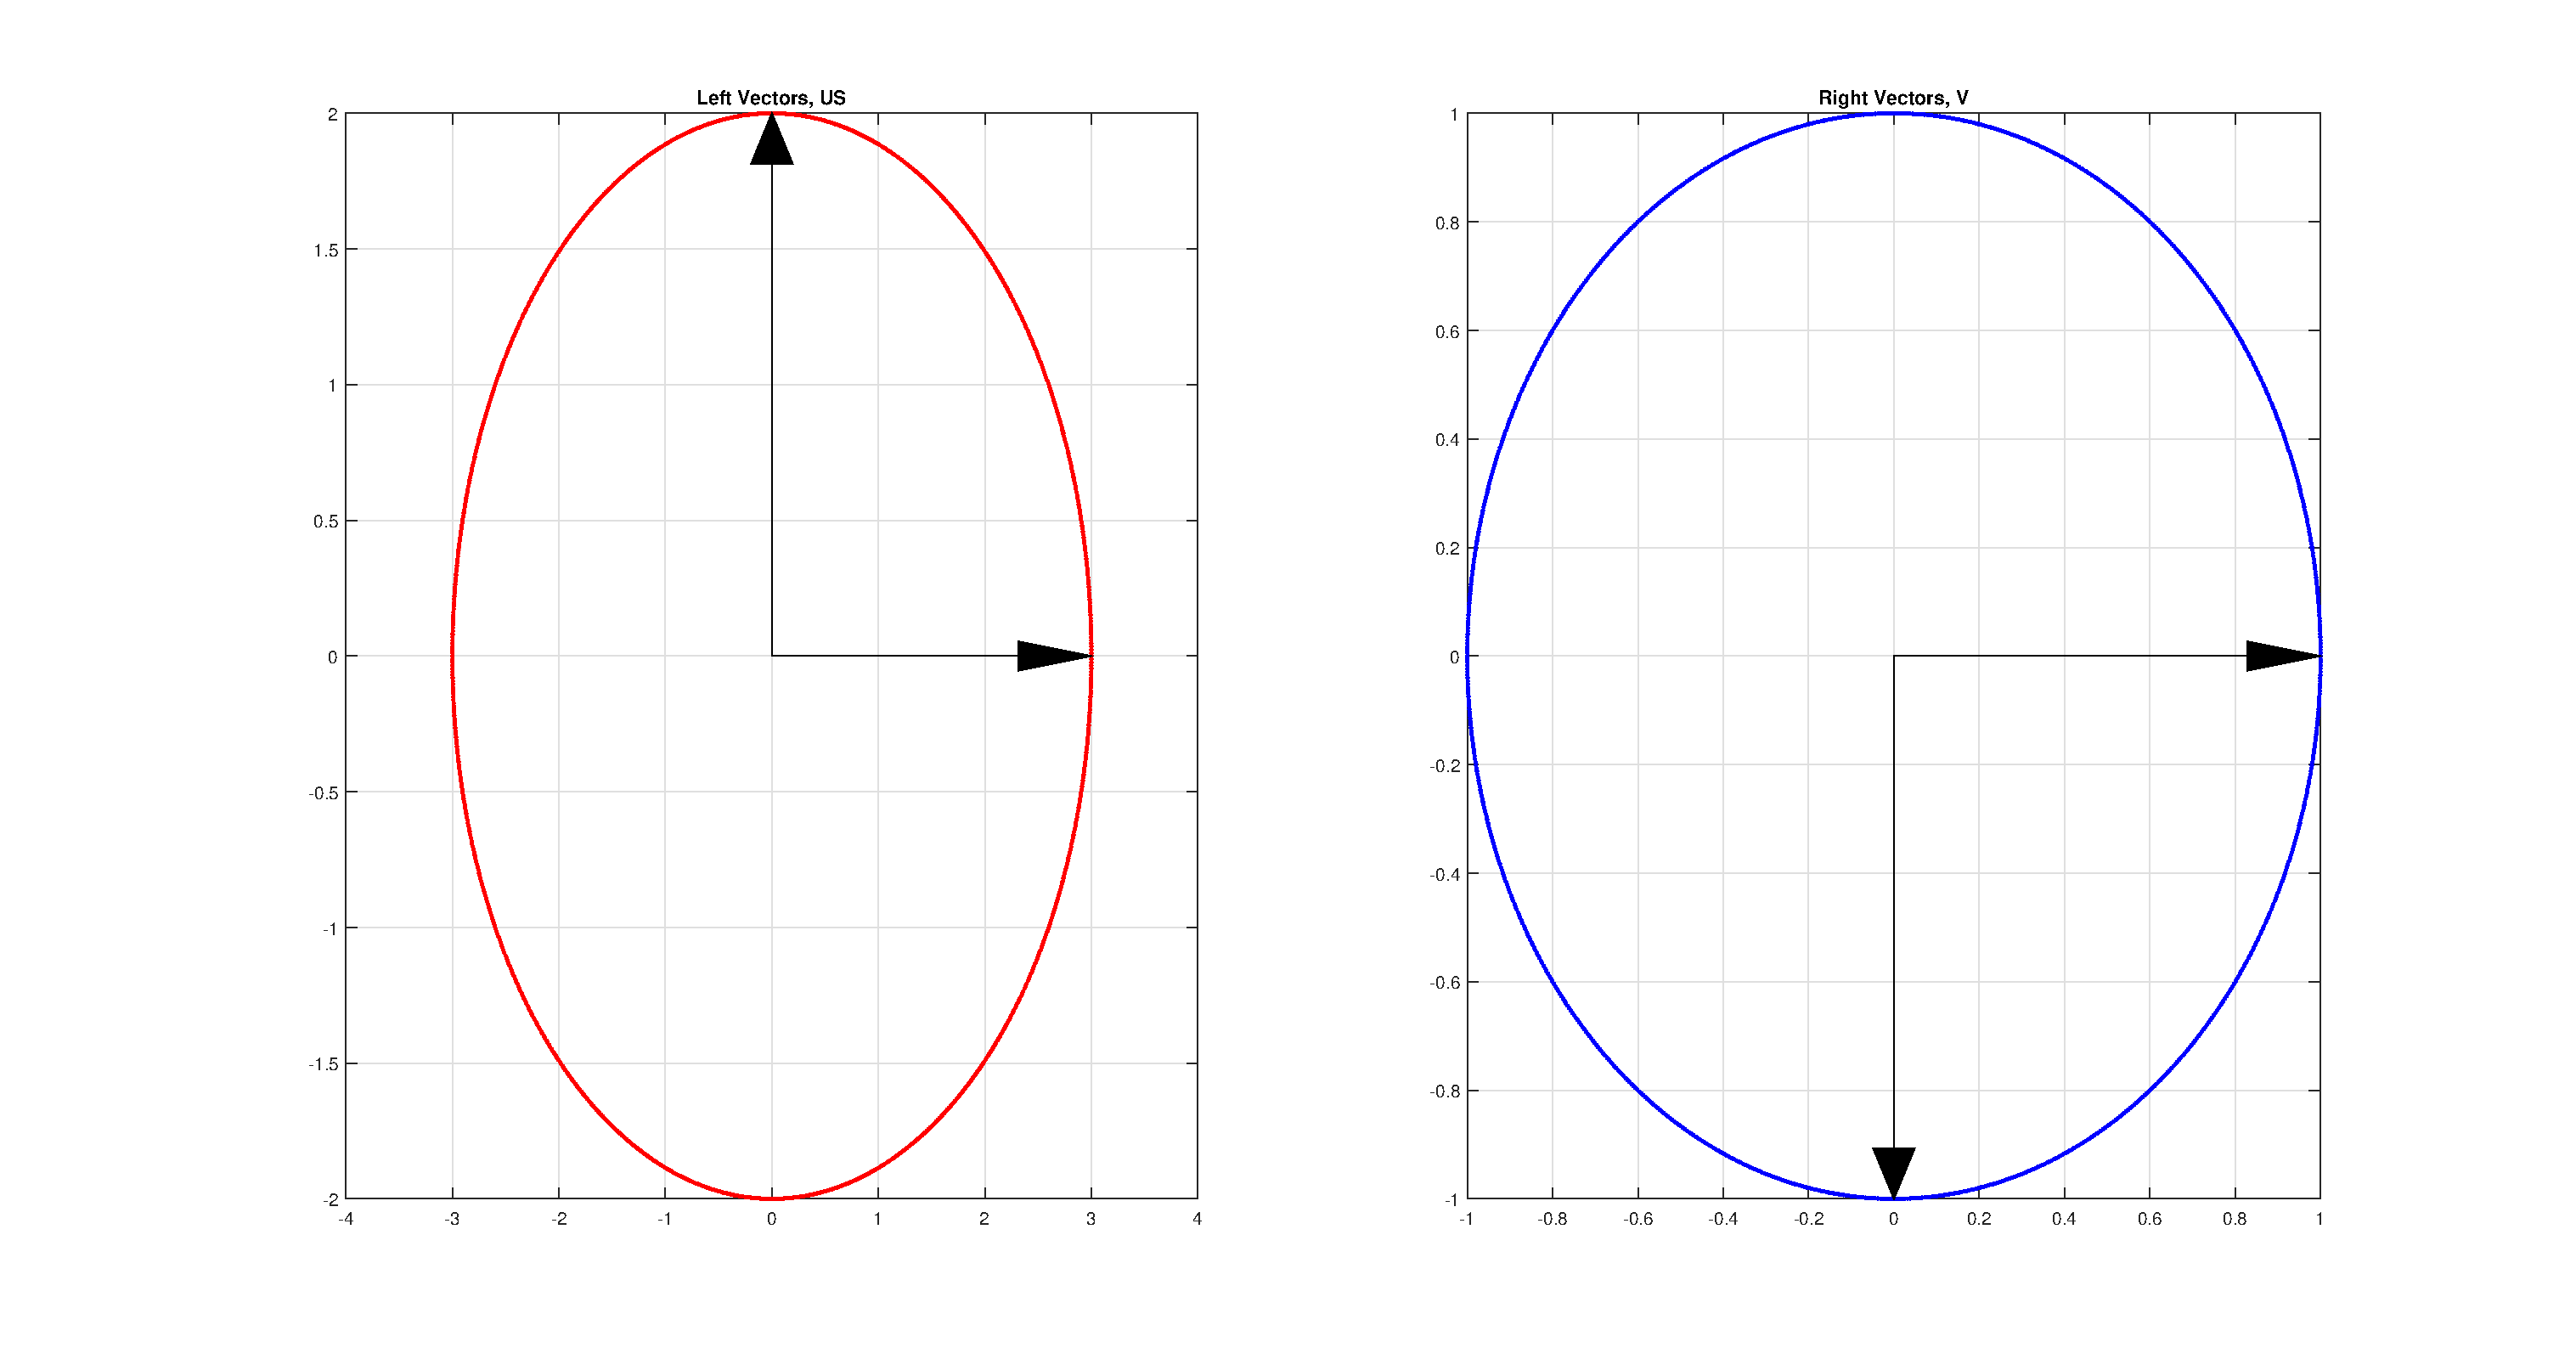
\includegraphics[width=9cm] {MatrixA} }} \\
		\subfloat[Matrix (b)]{{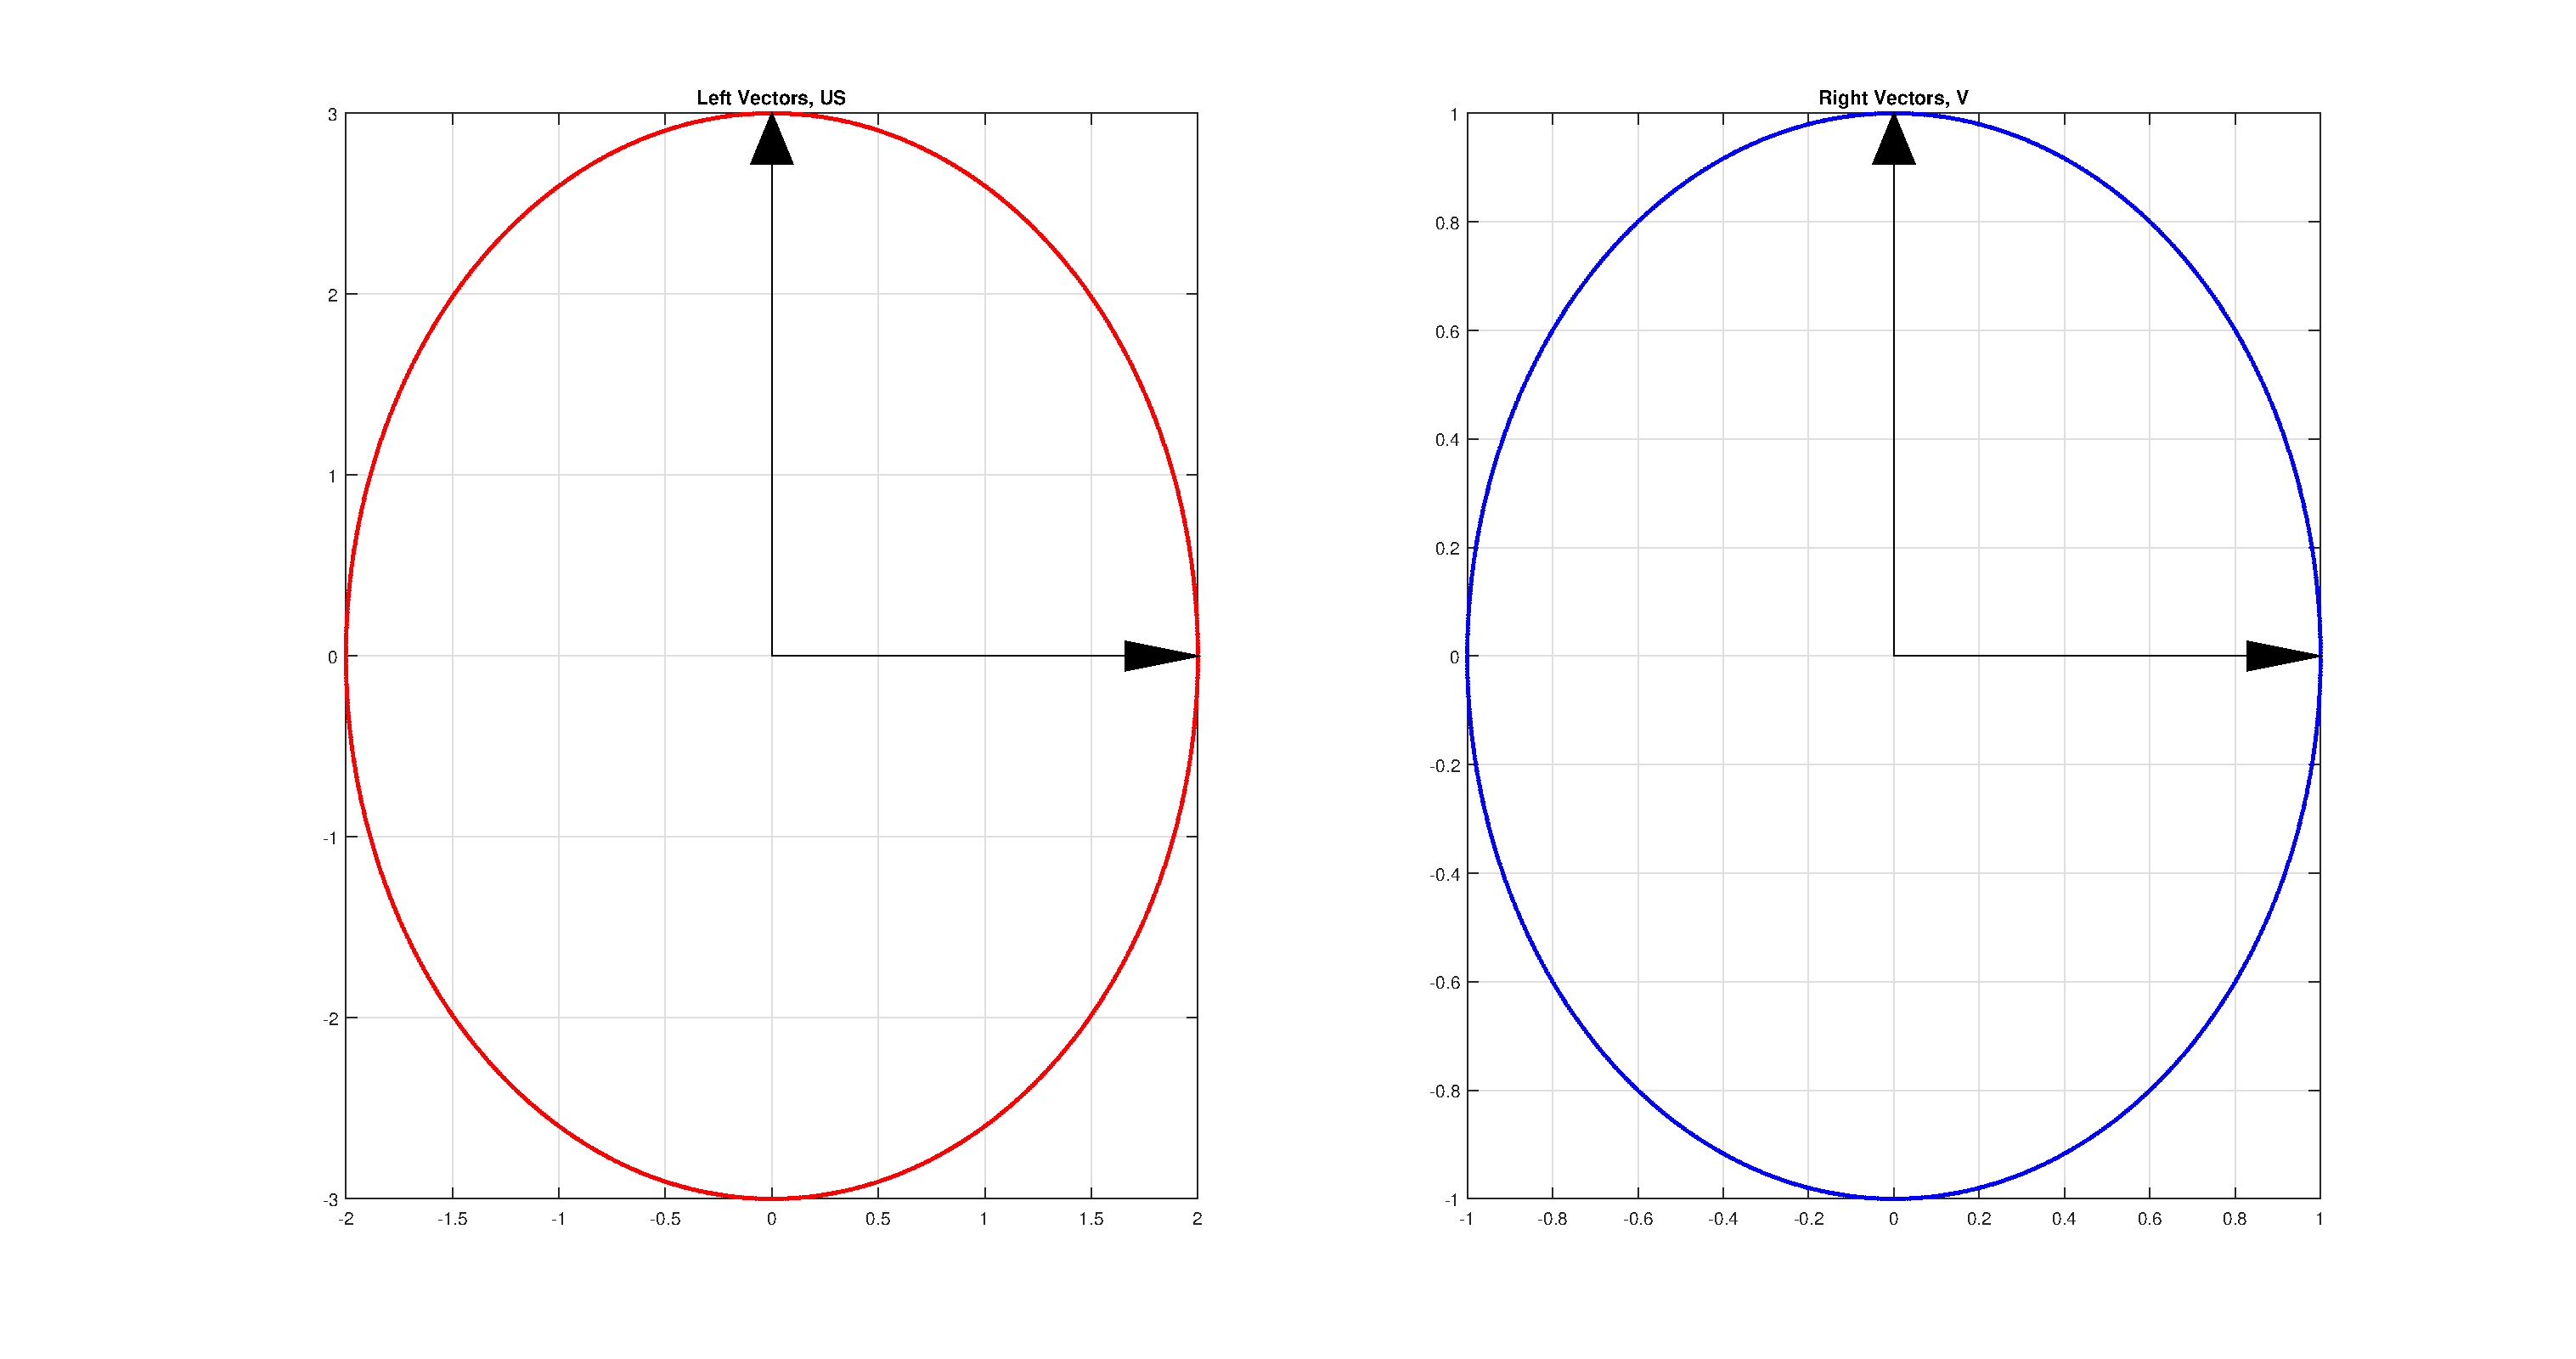
\includegraphics[width=9cm] {MatrixB} }}
		\subfloat[Matrix (d)]{{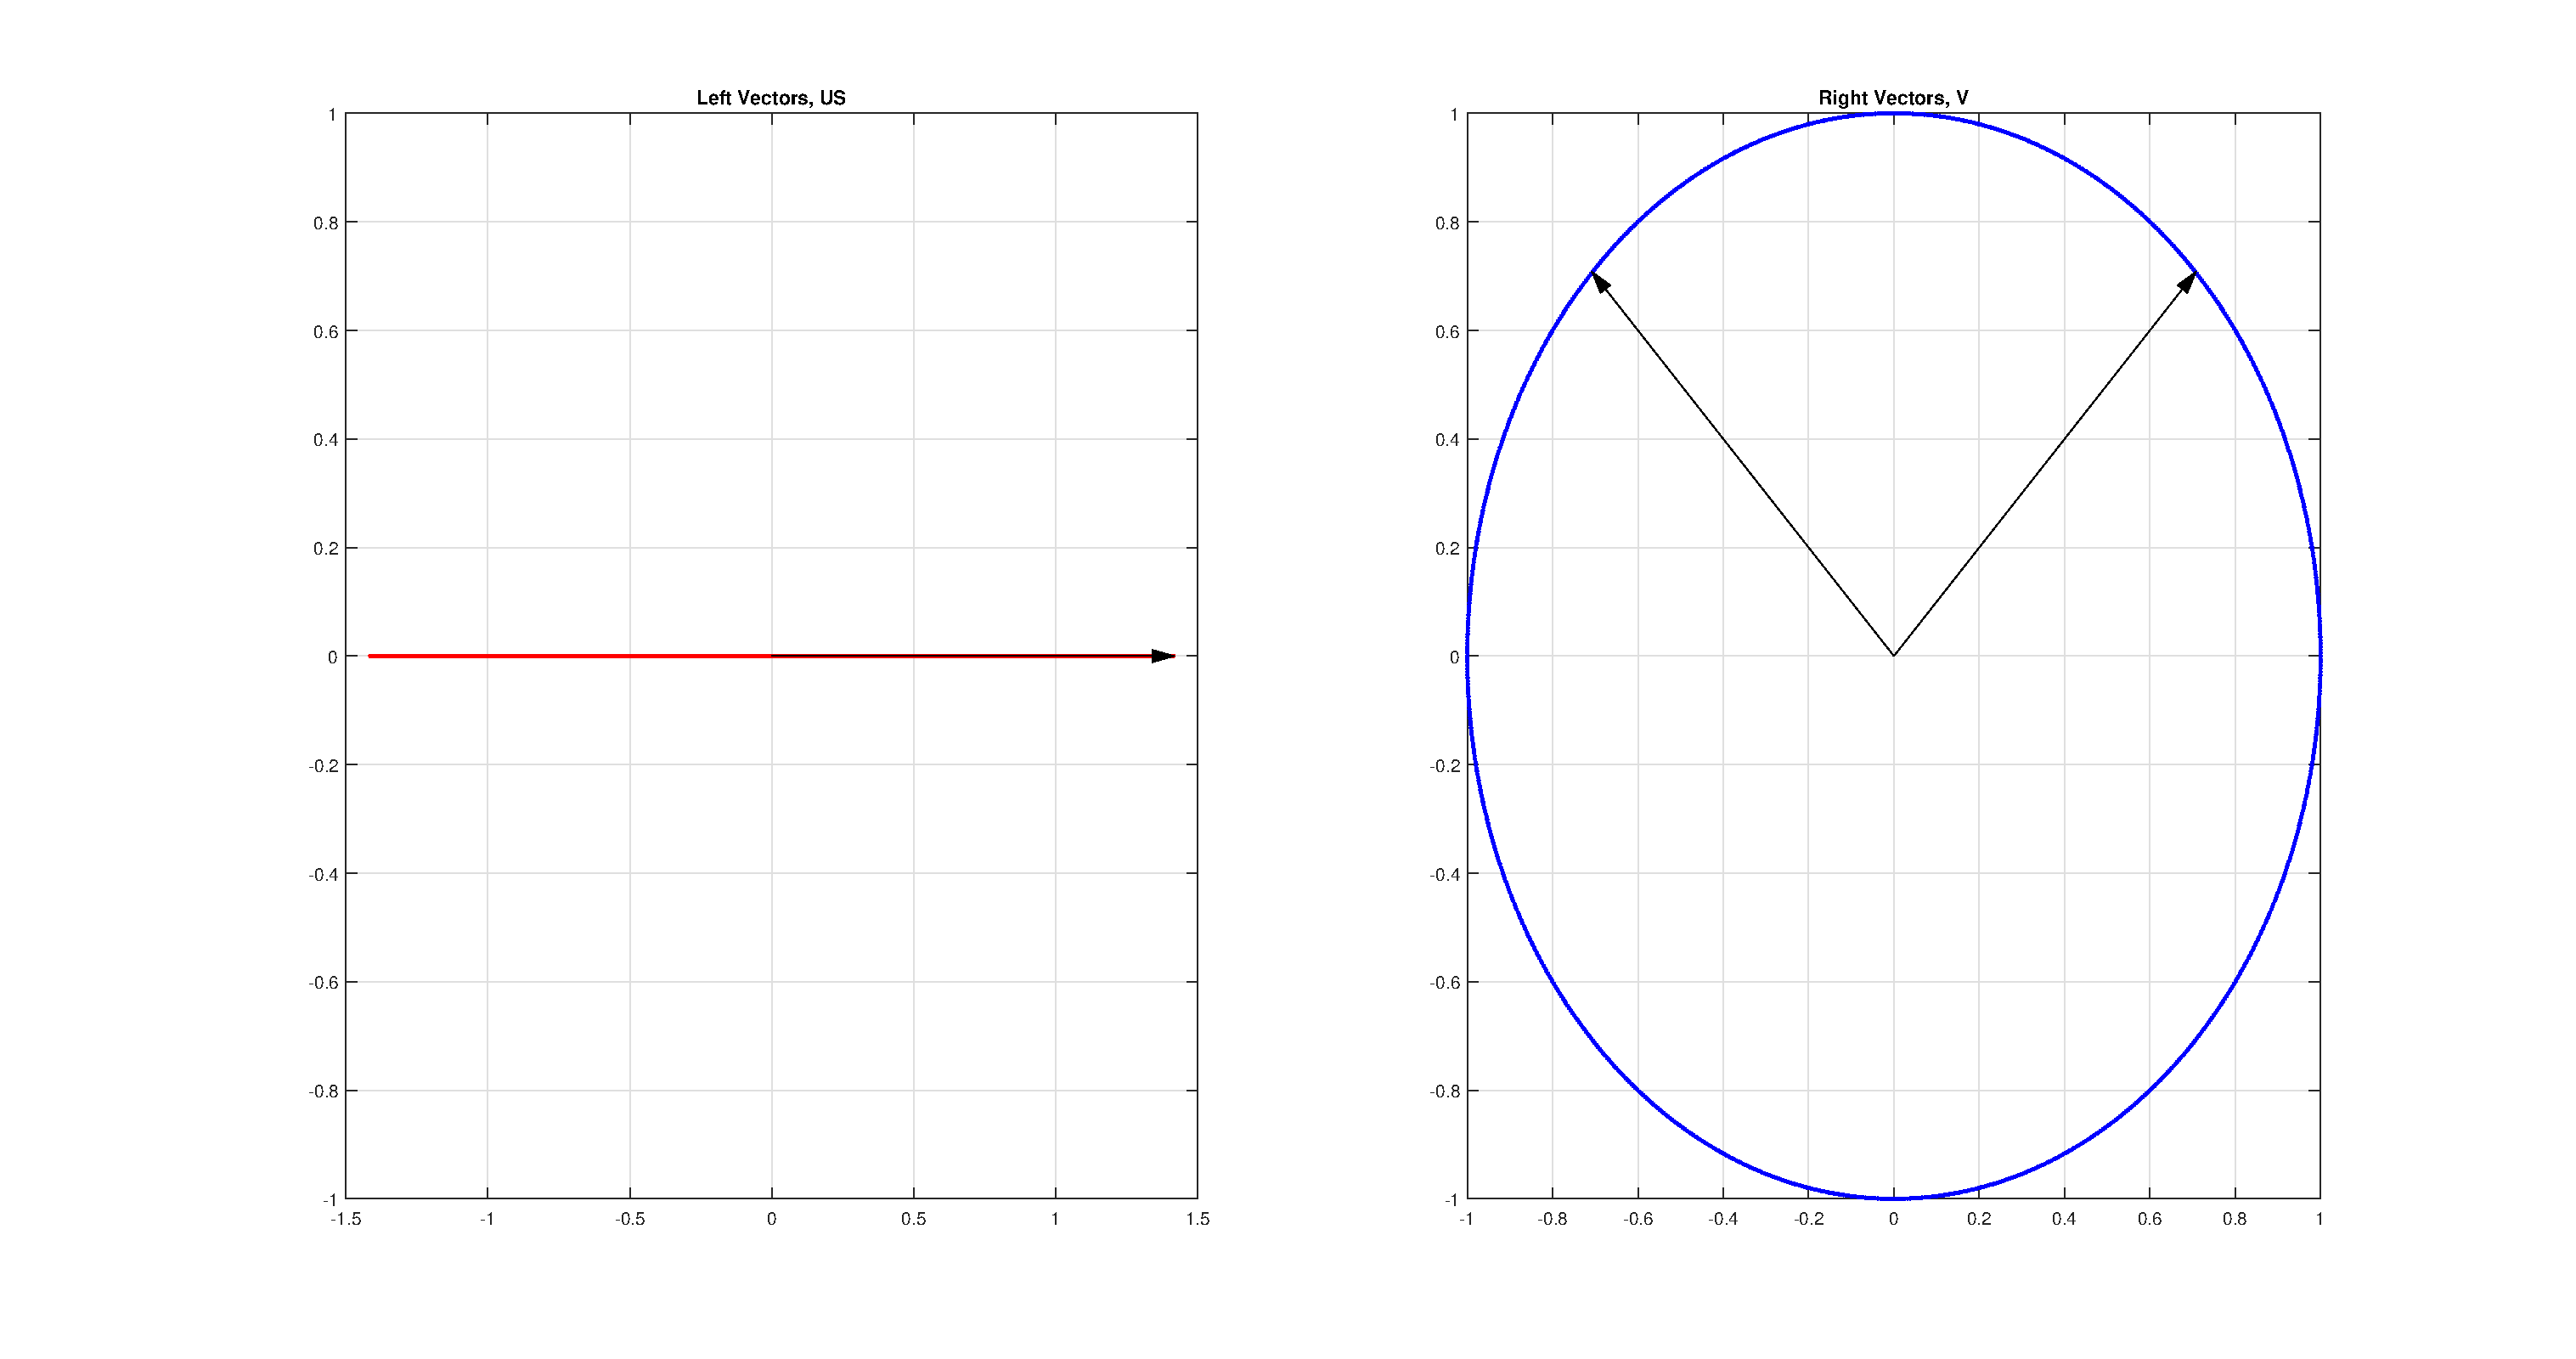
\includegraphics[width=9cm] {MatrixD} }} \\
		\subfloat[Matrix (e)]{{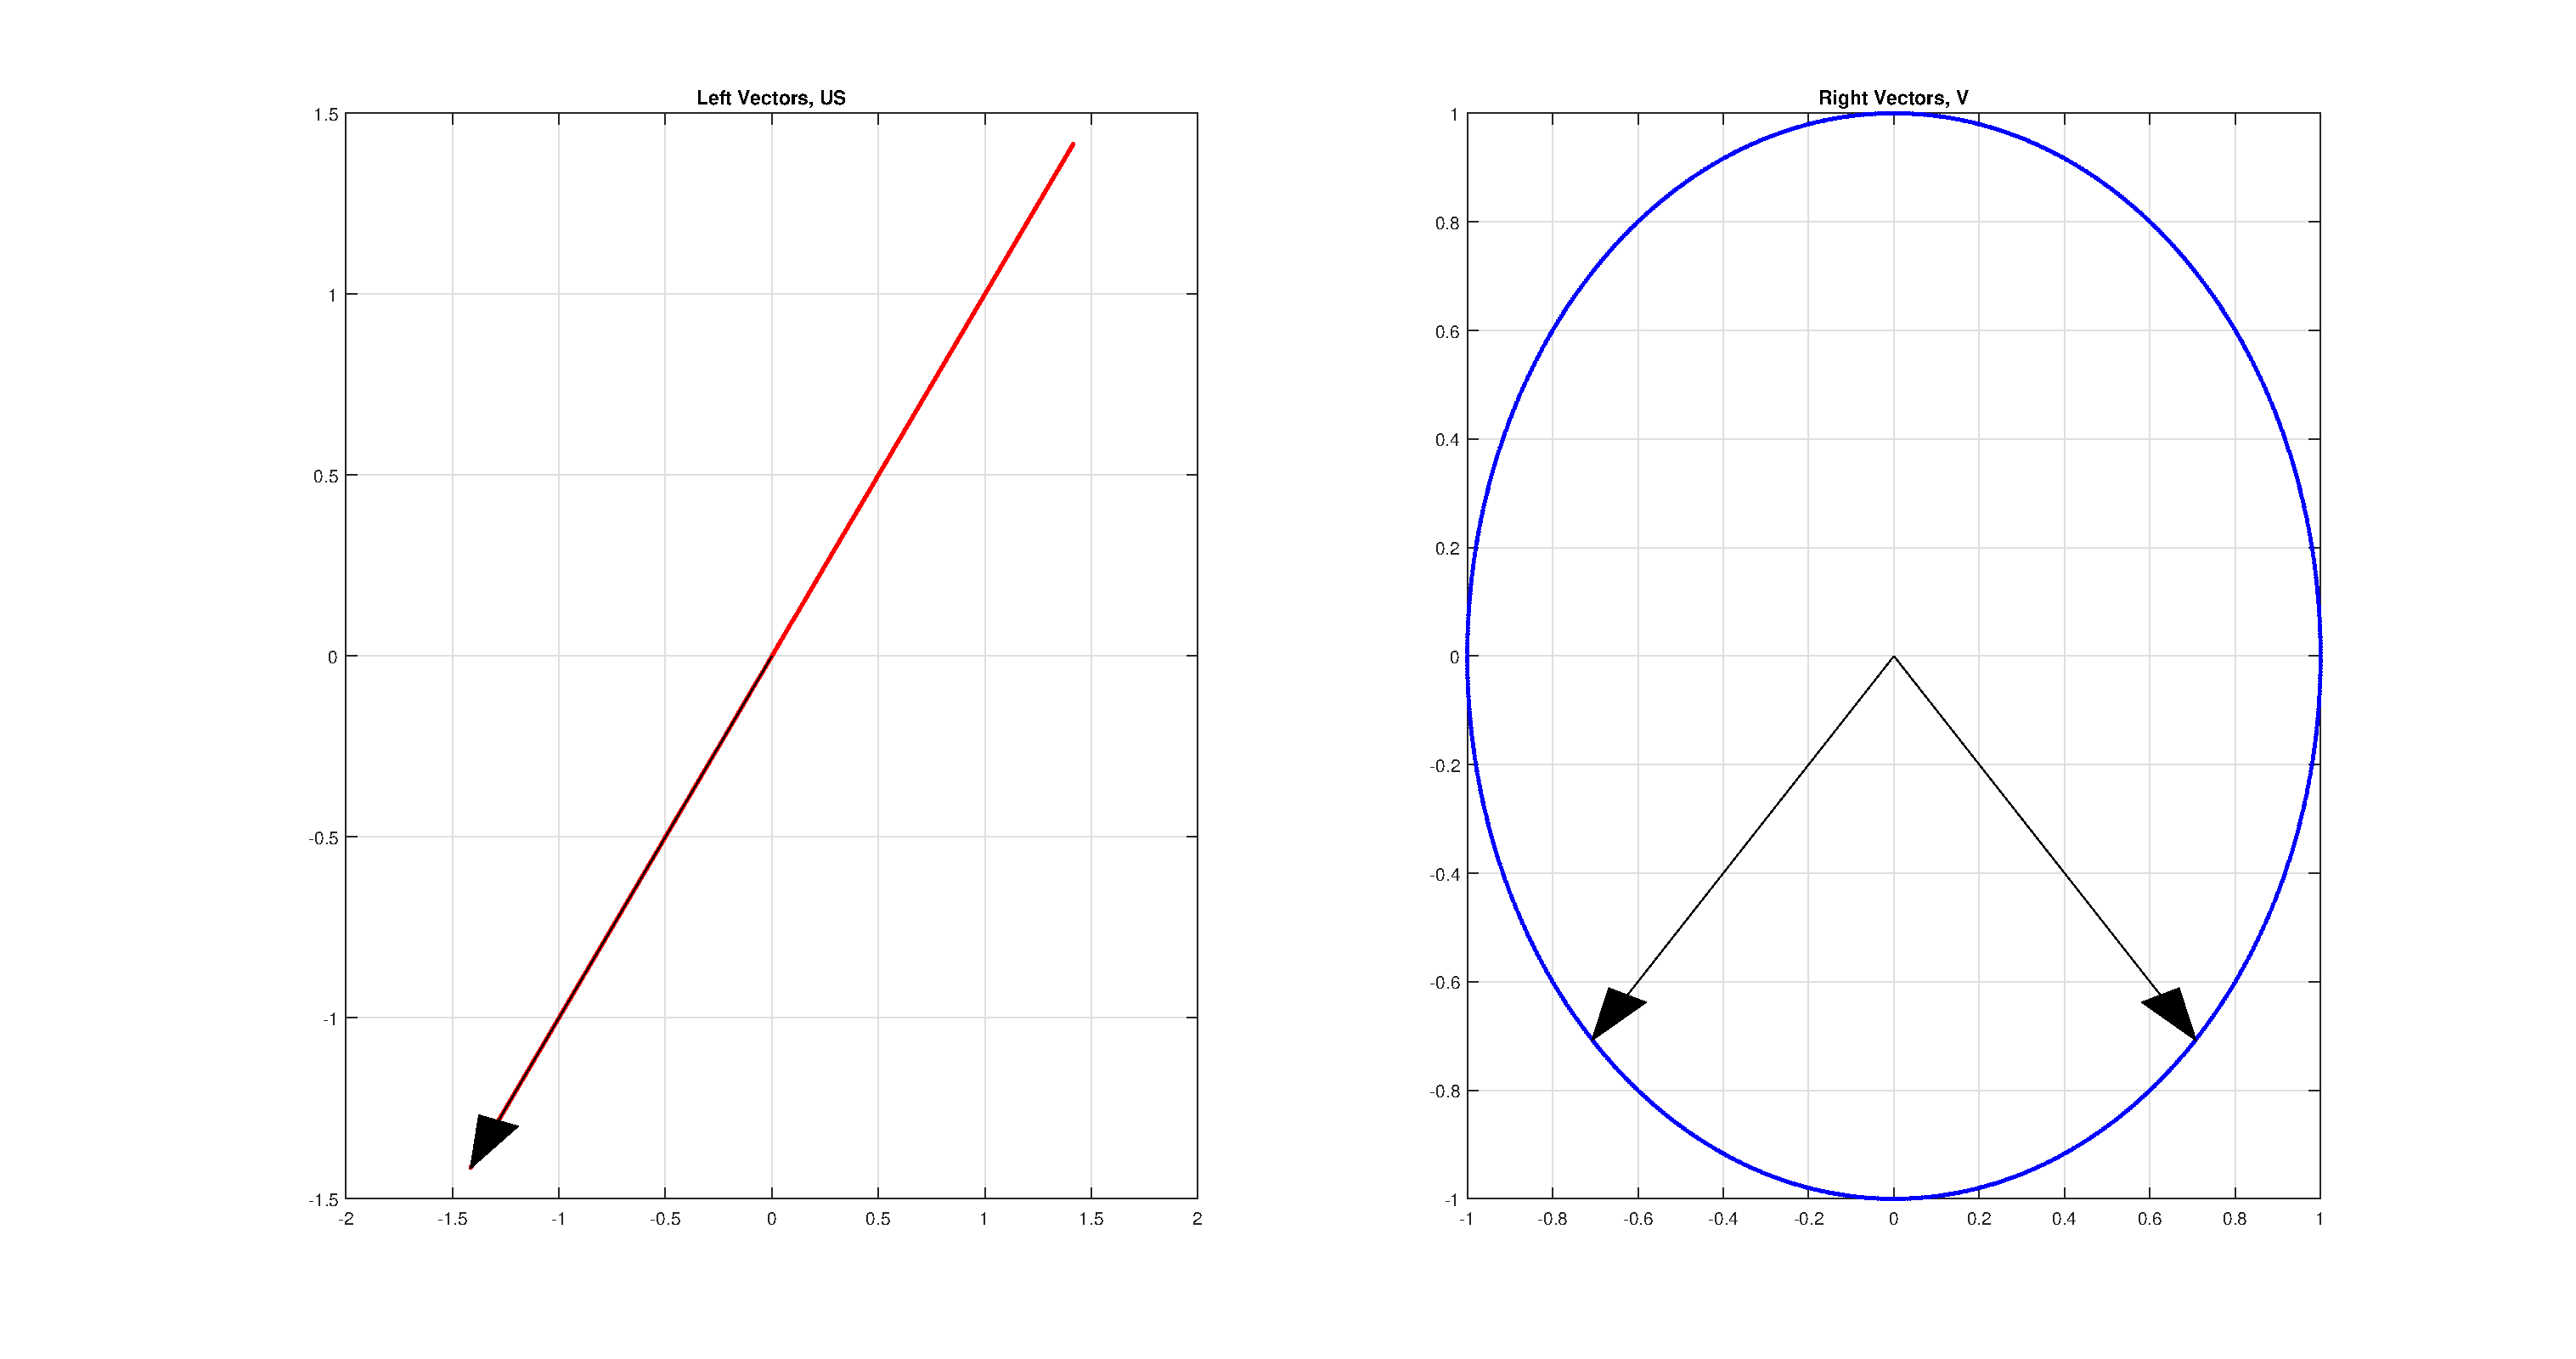
\includegraphics[width=9cm] {MatrixE} }}
	\end{figure}




\end{document}
